% TEMPLATE for Usenix papers, specifically to meet requirements of
%  USENIX '05
% originally a template for producing IEEE-format articles using LaTeX.
%   written by Matthew Ward, CS Department, Worcester Polytechnic Institute.
% adapted by David Beazley for his excellent SWIG paper in Proceedings,
%   Tcl 96
% turned into a smartass generic template by De Clarke, with thanks to
%   both the above pioneers
% use at your own risk.  Complaints to /dev/null.
% make it two column with no page numbering, default is 10 point

% Munged by Fred Douglis <douglis@research.att.com> 10/97 to separate
% the .sty file from the LaTeX source template, so that people can
% more easily include the .sty file into an existing document.  Also
% changed to more closely follow the style guidelines as represented
% by the Word sample file. 

% Note that since 2010, USENIX does not require endnotes. If you want
% foot of page notes, don't include the endnotes package in the 
% usepackage command, below.

% This version uses the latex2e styles, not the very ancient 2.09 stuff.
\documentclass[letterpaper,twocolumn,10pt]{article}
\usepackage{usenix2019,epsfig,endnotes,mathtools,bm,graphicx,subcaption,pdfpages,booktabs,mathrsfs,amsmath,amsthm,url,enumitem}

\begin{document}
%don't want date printed
\date{}


%Custom commands
\newcommand{\fref}[1]{\mbox{Figure~\ref{#1}}}
\newcommand{\secref}[1]{\mbox{Section~\ref{#1}}}
\newcommand{\tref}[1]{\mbox{Table~\ref{#1}}}


%\def\UrlBreaks{\do\/\do-\do:}

%Execution time
\newcommand{\exect}{\emph{Execution Metric}}
\newcommand{\name}{\emph{Blah}}

%make title bold and 14 pt font (Latex default is non-bold, 16 pt)
\title{\Large \bf Blockchain Structure Evolution}

%for single author (just remove % characters)
\author{
	Maria Papadaki\\
	Vrije Universiteit\\
	Amsterdam, The Netherlands\\
	m.papadaki@student.vu.nl
	\and
	Thodoris Zois\\
	Vrije Universiteit\\
	Amsterdam, The Netherlands\\
	t.zois@student.vu.nl
	\and
	Manuel Sanchez\\
	Vrije Universiteit\\
	Amsterdam, The Netherlands\\
	m.a.sanchezbernal@student.vu.nl
}

\maketitle

% Use the following at camera-ready time to suppress page numbers.
% Comment it out when you first submit the paper for review.
\thispagestyle{empty}

\subsection*{Abstract}

Plethora of goods and services provided by the Internet for exchange, have mandated the use of an anonymous payment system that does not pass through a central authority. The Bitcoin is the first of what we call cryptocurrencies and it is served by the Blockchain as its public transaction ledger. 
Over the last 10 years the Bitcoin gained a significant amount of users. Current statistics show that everyday almost 255.000 transactions are made.
Those transactions form a temporal graph and in this work we observe them and analyze the structure evolution of the Blockchain for each year, from 2009 until the March of 2017. For that reason, it is important to measure some critical and indicative for-the-graph metrics, such as Size, Diameter, Clustering Coefficient, Triangle Participation Ratio, Bridge Ratio and Conductance. Our findings show that the graph became an enormous chain of transactions data as the years passed by, with its size surged from 11.000 transaction to 4.8 billion at 2009 and 2015 respectively.

\subsection*{Keywords}
Bitcoin, Blockchain, Graph, Evolution, Structure, Metrics


\section{Introduction}
\label{sec:intro}

The factor that is decisive for this work is the emerged use of the Bitcoin for electronical exchanges. Unlike traditional currencies, Bitcoin keeps the identity of its owner hidden, it is easily portable, divisible, and irreversible. A decentralized digital currency without a central bank or single administrator are the words that characterize Bitcoin. It can be sent from user-to-user on the peer-to-peer Bitcoin network enabling the provision of financial services at a dramatically lower cost, and at the same time providing users more power and freedom~\cite{begginers}. The entire Bitcoin network relies on the Blockchain technology, a shared public ledger.

A Blockchain is a growing list of records that constitutes from blocks linked
together by using cryptographic techniques. Each block contains among other a
hash to the previous block, a timestamp, and a list of
transactions~\cite{wikiBlockchain}. A transaction is a transfer of value
between Bitcoin wallets. Those wallets keep a secret piece of data called a
private key or seed, which is used to sign transactions while providing a
mathematical proof that they have come from the owner of the wallet. The
signature also prevents the transaction from being altered by anybody once it
has been issued and keeps the identity of the user unknown~\cite{howworks}. 

All the transaction in the Blockchain are confirmed by the miners of the
network. Mining is the process of adding transaction records to the Bitcoin's
blocks. It is intentionally designed to be resource-intensive and difficult, so
that the number of blocks found each day by miners remain steady. The primary
purpose of mining is to set the history of transactions in a way that it is
impractical to modify by any one entity~\cite{wikiMining}. All transactions are
broadcast to the network and are usually confirmed within 10 minutes, where a
new block is created and added to the Blockchain.

An indication about the fame that Bitcoin gained over the years are some statistics from 2015 to 2018 that refer to the number of Blockchain wallet users worldwide. Since the creation of the Bitcoin in 2009 the number of Blockchain wallets has been growing reaching over 28 million at the end of September 2018. More specifically, in 2015 the number of Blockchain wallets was about 4 million, by the end of 2016 increased to 10 million while for 2017 to 17 million and at last, by end of 2018 it surged to almost 29 million wallets~\cite{statistics}.

Both the Bitcoin and the Blockchain are the object-of-interest of many studies, statistics and articles, that approach them from many different aspects in order to interpret data that come from either their own existance or from their analysis. Of course many of these studies are proposals that add a new dimension to Bitcoin or the Blockhain or even improve many different parts like the work of Ittay Eyal et al.~\cite{bitcoin-ng}.

The purpose of this work is to statistically analyze the Bitcoin Blockhain
structure evolution for each year, from 2009 until 2017. Due to the public
nature of the Bitcoin Blockchain, anyone can have access to the data and obtain
the complete history of transactions, which is approximately 98GBs. The key
concept of our analysis is that each block contains a UNIX timestamp that
allows us to split the transactions on certain time snapshots and form a
temporal graph with them. Using those graphs we compute metrics such as Size,
Diameter, Clustering Coefficient, Triangle Participation Ratio, Bridge Ratio
and Conductance, which are the pieces of a puzzle that provides us with a
complete image by visualizing them in order to conclude about 
the structure evolution for each year. 

The remainder of this manuscript is organized as follows. We begin by providing some background knowledge about the blocks and the transactions of the Bitcoin Blockchain as well as the metrics we compute in \secref{sec:background}. In \secref{sec:implementation} we describe the nature of our data, the tools that we use, the graph construction and the implementation of the algorithms. We describe our visualization types, and present our results in \secref{sec:results}. In \secref{sec:discussion} we discuss our approach, in \secref{sec:related} we survey related work and finally, in \secref{sec:conclusions} we conclude and address our future work.
 
\section{Background}
\label{sec:background}
The Blockchain is implemented as a chain of blocks where each one contains transactions. Blocks are created by users who are willing to use hardware resources in order to solve a computationally expensive mathematical problem which is unique for each block. Those users are called miners and once they verify the creation of a new block, the contained transactions are automatically approved and they get in return as a reward some Bitcoins. A block contains more than 500 transactions on average and its size can go up to 8MBs~\cite{damcosset}. 

The public nature of the Bitcoin Blockchain allows everyone to access the
complete history from the start and extract useful information. For instance,
one can indetify correlation patterns and trends or analyze the structure
evolution of the transactions graph, similar to our work. In the rest of this
section we provide some insight about the block and transaction schema as well as the
definitions of the metrics that we are going to compute for the transactions
graph.

\subsection{Block}
Every block in the Bitcoin network has the structure that ~\fref{fig:fig1} demonstrates. Each newly created block is chained to the last added and stores its digital fingerprint. The schema of the block is as follows:

\begin{itemize}
\item \textbf{Magic number (4 bytes):} This is an identifier for the Blockchain network. It has a constant value of 0xD9B4BEF9. It indicates the start of the block and that the data is from production network~\cite{medium}.

\item \textbf{Block size(4 bytes):} Indicates how large the block is.

\item \textbf{Version (4 bytes):} Mentions the Bitcoin protocol version that each node running on the network has to implement.

\item \textbf{Previous block hash (32 bytes):} It is a digital fingerprint (hash) of the \textit{block header} of the previous (last added) block of the Blockchain.

\item \textbf{Merkle Root (32 bytes):} A cryptographic hash of all of the transactions included in a block~\cite{architecture}.

\item \textbf{Timestamp (4 bytes):} The creation time of the block.

\item \textbf{Difficulty Target (4 bytes):} The current difficulty that was used to create this block.

\item \textbf{Nonce (4 bytes):} A random value that the creator of a block is allowed to manipulate.

\item \textbf{Transaction Counter (Variable: 1–9 bytes):} The number of transactions that are included within the block.

\item \textbf{Transaction List (Variable: Total block size is 1 MB):} Stores the digital fingerprint of all the transactions in that block.
\end{itemize}

Each block is characterized by a header. The \textit{Block header} is 80 bytes and it is composed by the fields from Version to Nonce.

\begin{figure}[htb]
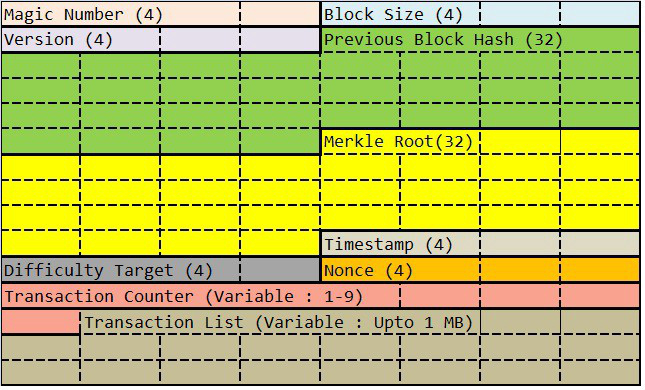
\includegraphics[width=1\linewidth]{./images/fig1}
\centering
\caption{The block structure. The number in the brackets is the size in bytes. Each individual cell is 1 byte. Hence, a field of 4 bytes occupies 4 cells. The fields from Version till Nonce are 80 bytes in total and form the \textit{block header}. Image source~\cite{medium}.}
\label{fig:fig1}
\end{figure}



\subsection{Transaction}
A Bitcoin transaction is the transfer or \textit{Bitcoins} from one address to another. Transferring does not mean physically moving an object from a source to a destination, but rather adding a new publicly accepted transaction entry to a block. Once a transaction is approved, it can never be removed or modified by anyone.

Transactions contain one-or-more inputs and one-or-more outputs. An \textit{input} is a reference to an output from a transaction in a previous block, whereas an \textit{output} specifies an amount and a address. Below we provide the abstract format of a Bitcoin transaction~\cite{mastering}:

\begin{itemize}
\item \textbf{Version (4 bytes):} Specifies which rules this transaction follows.
\item \textbf{Input Counter (1–9 bytes):} How many inputs are included.
\item \textbf{Inputs:} One or more transaction inputs.
\item \textbf{Output Counter (1–9 bytes):} How many outputs are included.
\item \textbf{Outputs:} One or more transaction outputs.
\item \textbf{Locktime (4 bytes):} A Unix timestamp or the block number.
\end{itemize}



\subsection{Metrics}
\label{label:metrics} The Bitcoin transactions can form a temporal graph in
which the transactions represent the edges of the graph and the Bitcoin
addresses represent the vertices. Based on this, we analyze the graph for each
year by computing some metrics that will provide us with an overall indication
of the structure. Below we provide the mathematical definition of each metric
that we compute later (Size, Triangle Participation Ratio, Bridge Ratio,
Clustering Coefficient, Conductance, Diameter) as well as the actual
information that these metrics provide for the structure of a graph in general.


\subsubsection{Size}
The size of the graph represents how big is the graph. It is the count of its total edges. In the following definition, ${\textstyle E}$ denotes the edges of the graph. 
\begin{align*}
  Sz &= \vert E \vert\\
\end{align*}



\subsubsection{Triangle Participation Ratio}
Triangle Participation Ratio (TPR) is a metric that for each vertex counts in how many triangles it participates in. In the following definition ${\textstyle t(x,S)}$ is the number of triangles that vertex ${\textstyle x}$ closes with-and-only-with the vertices in set ${\textstyle S}$.

\begin{align*}
  TPR &= \frac{\vert{\{x\in S : t(x,S) > 0 \}}\vert}{\vert S\vert}\\
\end{align*}



\subsubsection{Clustering Coefficient}
Clustering Coefficient is the measure of the degree to which nodes tend to cluster together. Three versions exist: the Global, the Local and the Average~\cite{cc}. 

Global Clustering Coefficient is designed to give an overall indication of the clustering in the network. In the following definition ${\textstyle tri(G)}$ is the number of triangles of a graph and ${\textstyle t(G)}$ is the number of the open and closed triplets.
\begin{align*}
  G\_CC &= \frac{ 3 \times tri(G) }{ t(G) }\\
\end{align*}

Local Clustering Coefficient provides an indication of the embeddedness of single nodes. It quantifies how close the neighbours of a vertex are to being a clique (complete graph). The Local Clustering Coefficient for a vertex ${\textstyle v_i}$ is given by the proportion of links between the vertices within its neighbourhood divided by the number of links that could possibly exist between them. For a directed graph, ${\textstyle e_{ij}}$ is distinct from ${\textstyle e_{ji}}$,  and therefore for each neighbourhood ${\textstyle N_i}$ there are ${\textstyle k_i (k_i - 1)}$ links that could exist among the vertices within the neighbourhood. In the following definition ${\textstyle k_i}$ is the number of neighbours of a vertex and ${\textstyle E}$ represent the edges of the graph.
\begin{align*}
  L\_CC &= \frac{\vert{\{e_jk : v_j,v_k \in N_i ,e_jk \in E\}}\vert}{k_i (k_i - 1)}\\
\end{align*}

Average is the mean of the Local Clustering Coefficient of all the vertices ${\textstyle n}$. The definition is as follows:
\begin{align*}
  \overline{L\_CC} &= \frac{1}{n} \sum_{i=1}^{n} C_i\\
\end{align*}



\subsubsection{Conductance}
The Conductance measures how "well-knit" is the graph. It controls how fast a random walk on ${\textstyle G}$ converges to a uniform distribution. Low Conductance means good clustering for the graph. The Conductance of the whole graph is the minimum conductance of all the possible cuts. In the following definition the cut of the graph is ${\textstyle (S,\overline{S})}$ and ${\textstyle \alpha_{ij}}$ are the entries of the adjacency matrix.
\begin{align*}
 	C &= \displaystyle\min_{S \subseteq V} ( \frac{\sum_{i \in S,j \in \overline{S}} \alpha_{ij} }{\min ( \alpha (S), \alpha ( \overline{S} ) )} ) 
\end{align*}



\subsubsection{Bridge Ratio}
Bridge ratio is the fraction of bridges to the total number of edges and its purpose is to show the vulnerabilities of a graph. A bridge is defined as an edge whose deletion disconnects the graph. In the following definition ${\textstyle N(x)}$ is the set of neighbors of ${\textstyle x}$ and ${\textstyle S}$ the set of vertices.
\begin{align*}
  BR &= \frac{bridges(S)}{\sum_{\mkern-5mu x\in S \vert{N(x)\cap S}\vert}}\\
\end{align*}



\subsubsection{Diameter}
Diameter is another measurement for the structure of a graph. It measures the topological length or extent of a graph by counting the number of edges in the shortest path between the most distant vertices~\cite{diameter}. Diameter is the maximum from all the shortest paths. In the following definition ${\textstyle s(i, j)}$ is the number of edges in the shortest path from vertex ${\textstyle i}$ to vertex ${\textstyle j}$.
\begin{align*}
  D &= \max(s(i,j))\\
\end{align*}

\section{Implementation}
\label{sec:implementation}

The Bitcoin Blockchain for the period of 2009 until March of 2017 constitutes
from blocks with a total size of approximately 98GBs. We analyze the data using
Apache Spark~\cite{Zaharia} with Scala and an open-source tool that integrates
very well with Spark, HadoopCryptoledger~\cite{cryptoledger}. HadoopCryptoLedger 
provides us with the ability to form the block and transaction objects as well as 
an example on how to construct the transactions graph. Since we have to do graph-processing
to compute our metrics we need a tool that cooperates impeccable with Apache
Spark in parallel and distributed computing; thus, the use of
GraphX~\cite{graphx} is decisive. After computing the metrics, we create
interactive visualizations of the results into a Bootstrap~\cite{bootstrap}
HTML website using Chart.js~\cite{chartjs}. We use \textit{Bar Charts} to represent the years, \textit{Line Charts} for the months of each yearand one \textit{Pie Chart} for the Size that demostrantes the contributed percentage of 
each year to the total of the graph. For the visualization of the
community that provides the Conductance of the graph, we use gexf-js.js~\cite{gexfjs}
which cooperates well with Gephi~\cite{gephi} and allows us to visualize the results into the website. 
We store all the data of the Bitcoin Blockchain into HDFS and we compute the metrics on a small part of the Dutch
national e-infrastructure with the support of SURF Cooperative.

\begin{figure*}[h!]
	\centering
	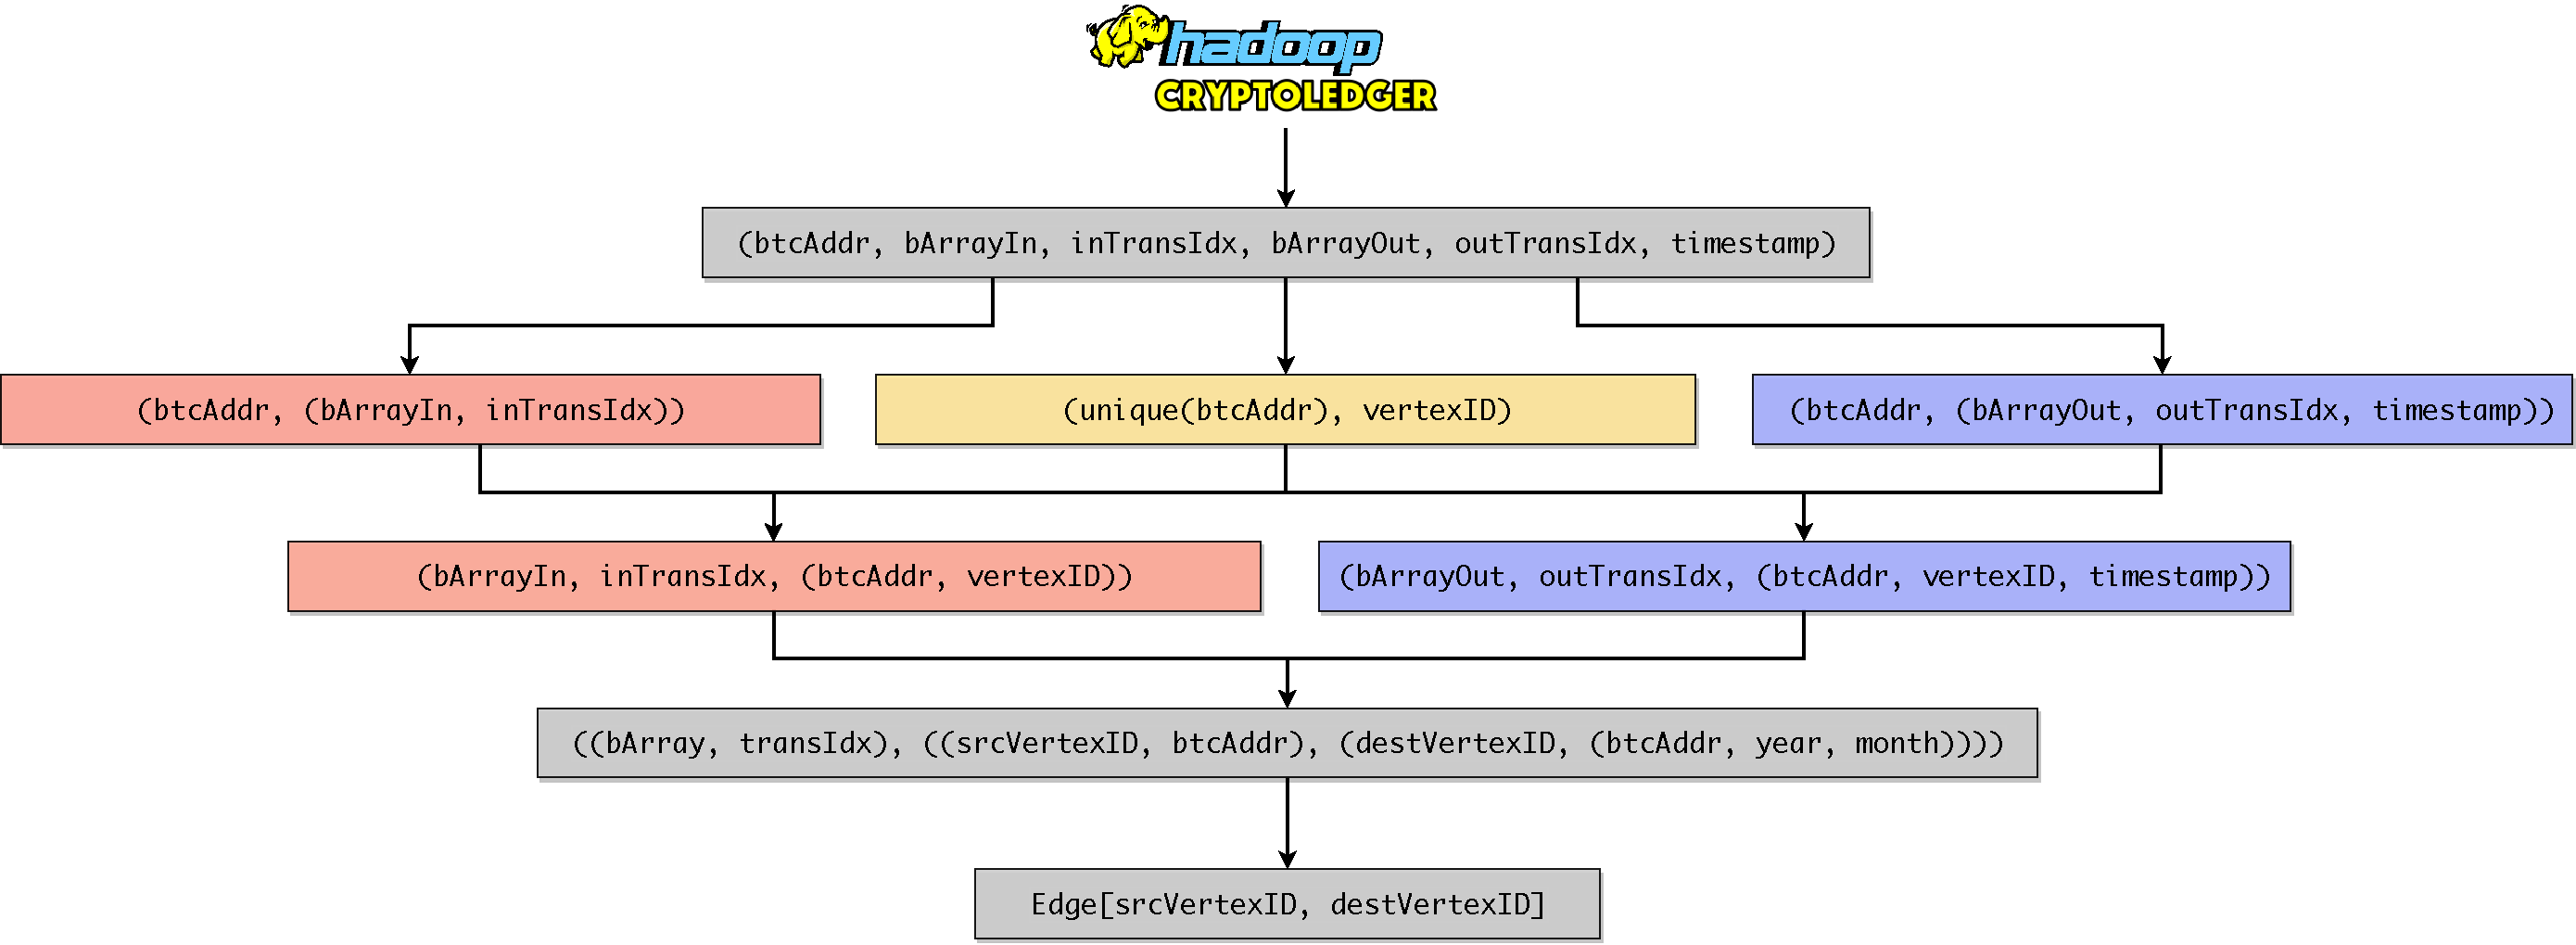
\includegraphics[width=1\linewidth]{./images/fig2}
	\caption{The steps of producing the edges of the graph. We construct the graph only from the edges and we only the source and destination vertex ID from the final results of the process. Hence, we keep those as well as the timestamp which we convert to date in order to partition the graph to different timesnapshots.}
	\label{fig:fig2}
\end{figure*}

\subsection{Transactions Graph}
The foundations of this work is the great size of our data and how we treat them. Our dataset consists of 98GBs of Bitcoin Blockchain blocks. Since the amount of data is big enough to use them for the metrics computation without any pre-processing, we filter out everything that we do not need. As we describe in~\secref{sec:background} each block in the Blockchain contains numerous information, but for the purposes of our analysis we only need the timestamp and the transactions list. Our approach to represent the graph, is that every Bitcoin address is a vertex and every transaction is a directed edge from one vertex to another.

Each transaction in the list is constructed from input and output transactions,
where the input transactions come from previous blocks. HadoopCryptoledger
deserializes the blocks and iterates through each transaction entry in the list
and returns the \textit{destination Bitcoin address}, the \textit{input} and \textit{output ByteArray} and the \textit{index of the input} and 
\textit{output transaction} in the list. However, the timestamp of the block is missing. Thus, we modify the
code and we add it to the returning results. 

Since the Bitcoin addresses represent the vertices in a graph, we gather all
the unique addresses, we store them into an RDD and we assign them a vertex ID.
To construct the edges, we need to join all the input with the output
transactions. First, we construct the input and output transactions RDDs and we assign the timestamp
only to the output transaction to avoid confusion of the dates coming from
previous blocks after the join. For instance, if we assign the timestamp to
both, we can end up with the input transaction date being later than the
output, which is impossible since the input transactions come from previous
mined blocks.

Before joining the input and output RDDs to obtain the edges, we first need the
vertex ID on each row of both RDDs since it will represent the source and
destination of our edge. Hence, we join each RDD with the one that contains the
unique Bitcoin addresses. We then join the results on
the ByteArray and the transaction index and we end up with the edges for the
graph. However, we do not need neither all the information of the results nor
the vertices, since we can construct the graph only from the edges. Thus, we
discard everything and we keep only the timestamp and the source and
destination vertex ID. Finally, we convert the final RDD into a DataFrame in
order to convert the timestamp to date and partition the graph on certain time
snapshots. We keep only the year and month columns and we partition the edges
by them storing the results into HDFS as parquet files. Each time, not only we
are able to load the graph for the desired timesnapshot but also we manage to
reduce the size of the data from 98GBs to 14GBs.~\fref{fig:fig2} demonstrates
the procedure described above.


\subsection{Metrics Implementation}

Based on the formulas described in \secref{sec:background} we implement our
algorithms in Scala by the agency of GraphX which provides several functions
for graph-processing~\cite{graphxDoc}. The metrics that we compute are mostly
iterative algorithms that need a lot of time as the size of the graph increases each year. 
Below we describe the methodology that we follow in order to
compute each metric, as well as some functions of GraphX that proved to be really handy.

\subsubsection{Size}
Computing the Size of a graph is simple process as we just need to count the total number of edges. We use the function \textit{Graph.numEdges} that GraphX provides.

\subsubsection{Triangle Participation Ratio}
For the Triangle Participation Ratio the proccess we follow is to find the total number of vertices that participate in a triangle. For this step we use the function \textit{Graph.triangleCount} of GraphX, we filter out the vertices that do not participate in any triangle and then, we divide the result with the total number of vertices of the graph.

\subsubsection{Bridge Ratio} Our approach to compute Bridge Ratio is to use the
DFS traversal algorithm with a complexity of O(V\texttt{+}E). The main idea is
to keep track of the visited vertices by finding the neighbors of each vertex,
go through them, and store parent vertices in a DFS tree. In order to find the
neighbors of each vertex we use the \textit{Graph.collectNeighborIds} function from
GraphX. Then, we check if the subtree rooted with the current neighbor of the
vertex has a connection to one of the ancestors of the specific vertex. If the
lowest vertex reachable from the subtree under the specific vertex is below its
parent vertex in the DFS tree, then the edge that connects the current 
and its parent vertex is a bridge.

\subsubsection{Global Clustering Coefficient}
For the Global Clustering Coefficient, the urgent matter is to compute the total number of triangles as well as the total number of open and close triplets. For that reason, we use the functions \textit{Graph.trianglesCount} and \textit{Graph.triplets} of GraphX, to compute respectively each of the above. Then, we multiply with 3 the number of triangles and divide them by the total number of triplets.

\subsubsection{Conductance}
To compute Conductance, we first need to generate the K non-overlapping cuts. For that reason we apply the \textit{Label Propagation} algorithm in order to split the graph into communities. We perform 10 iterations and then we discard the communities containing less than 10 edges since their importance compared to the size of other communities has minor importance for the result. As we further analyze in~\secref{sec:discussion}, due to the complexity of the computation, we choose only the top 10 communities in edgs for the computation. For those communities we compute the fraction of edges going out to the minimun total edges and we report the minimum of those values.

\subsubsection{Average Clustering Coefficient \& Diameter}
In order to compute the Average Clustering Coefficient, we use the implementation of Sherlock Yang~\cite{localCCgit}, that computes the Local Clustering Coefficient for each vertex. The Average Clustering Coefficient derives from summing the results and finding the mean value. In addition, the Diameter implementation is equivalent with the one derivered from~\cite{diam1, diam2} and can be found on publicly available at GitHub~\cite{diamGit}.


\section{Results}
\label{sec:results} 

Our work aims to analyze the evolution of the Bitcoin Blockchain on certain
time snapshots. Our data are of a high quality since they are generated from a
controlled environment and hence they do not include any noise. They range from
2009 until the March of 2017 and are approximately 98GBs, which we finally
manage to reduce to 14GBs of parquet files. We perform our computations for
each year individually and we do not count the results of previous years in
order to compute a metric for the next. Our analysis is based on years and
months, however we limit the amount of visualizations in the present manuscript
for reader's-ease reasons. We choose to discuss the results only for the years
as those are sufficient for comparisons and conclusions. In our
website~\cite{website} we provide also visualizations of the results per month
of each year, as well as the graph visualizations of the communities that produced the 
minimum Conductance, hence the Conductance of the whole graph. 


\subsection{Size}
\fref{fig:fig3} represents the evolution of the graph for each year in terms of size. As we refer in~\secref{sec:background} the size of the graph is conducted from the number of edges. Since each edge on the graph represents a transaction, we observe that the transactions continuously rose per year.
For 2009 the number of transactions was 22.000 while for 2015 reached a peak with 4.8 billion.

\begin{figure}[h!]
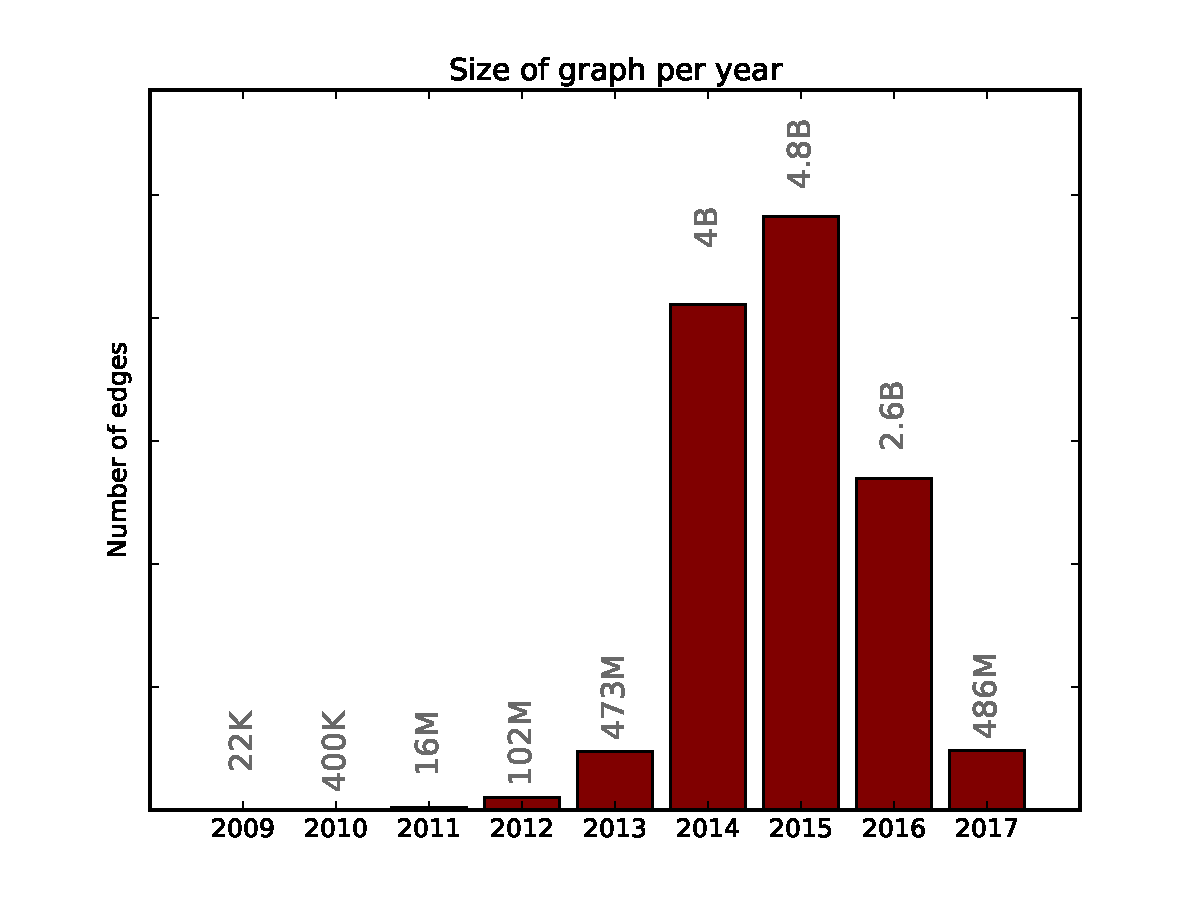
\includegraphics[width=1\linewidth]{./images/size}
\centering
\caption{The size of the graph per year. Since the size is conducted from the number of edges and the edges in the graph represent transactions, we observe that transactions in the Bitcoin Blockchain continuously increased. The peak is in 2015 where 4.8 billion transactions take place.}
\label{fig:fig3}
\end{figure}


\subsection{Triangle Participation Ratio}
\fref{fig:fig4} demonstrates the clustering of the graph through Triangle Participation Ratio. For the years 2009 to 2012 there is a fluctuation which later becomes a constant decrease until the March of 2017 that reaches the half of the value of 2012. We interpret the TPR as transactions between cliques. The decrease of TPR after 2012 was expected due to the size of the graph that starts increasing dramatically, hence the transactions become more spread between users. Generally, we observe that the TPR does not exceed 37\% for any of the years which indicates the lack of small communities compared to the total size of the network.


\begin{figure}[h!]
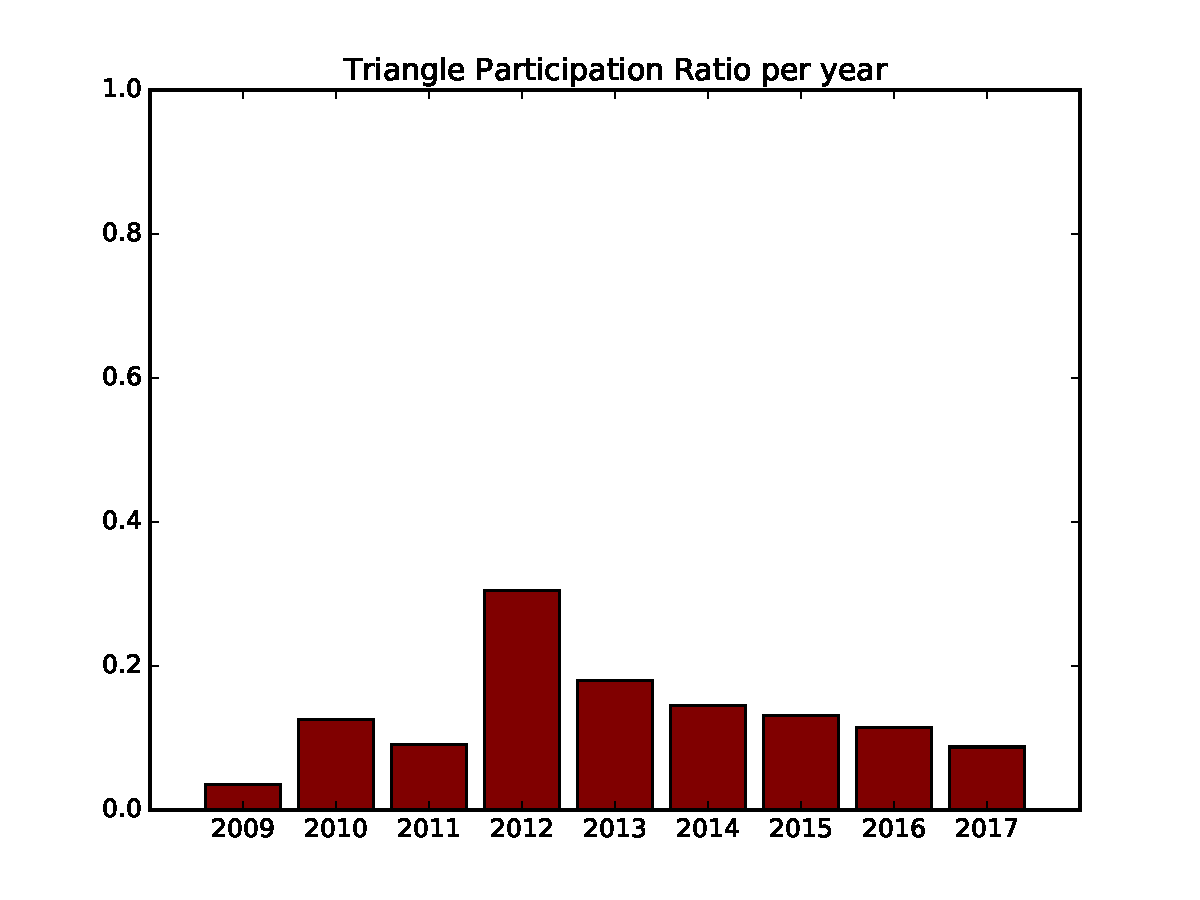
\includegraphics[width=1\linewidth]{./images/tpr}
\centering
\caption{The Triangle Participation Ratio of the vertices for each year from 2009 until March of 2017. From the results we can observe that in general the ratio is pretty low which is interpreted as the difficulty of existance of small societies in a large graph.}
\label{fig:fig4}
\end{figure}

\subsection{Clustering Coefficient}
When we turn to analyze the Clustering Coefficient, as~\fref{fig:fig5} shows,
we can observe that the Average Clustering Coefficient for each year is between
0 and 0.1. This ratio indicates that there are only a few vertices that their
neighbors form a clique and we can correlate it with the low Triangle
Participation Ratio.

On the other hand, the Global Clustering Coefficient has greater values than the Average. The distribution of the ratio is between 0.04 and 0.7 with the second one being a peak in 2011 followed by 2012 with a ratio around 0.65. From those two results we can comprehend that a high number of closed triplets existed in each graph and hence the clustering of those two individual years was very good compared to others. However, as a general conclusion most of the years do not have a good clustering between transactions.

\begin{figure}[t]
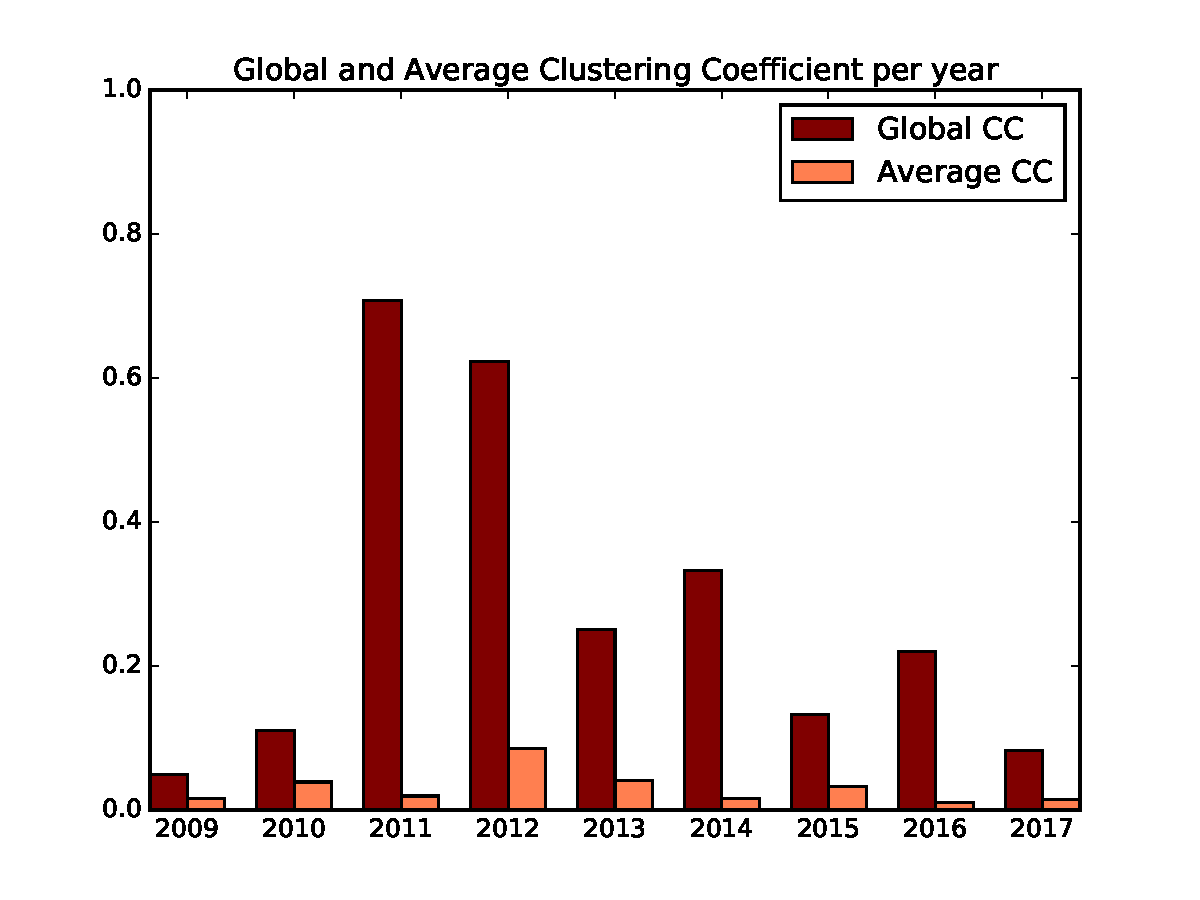
\includegraphics[width=1\linewidth]{./images/cc}
\centering
\caption{The Global and the Average Clustering Coefficient of the graph for each year from 2009 until March of 2017. The years 2011 and 2012 have the highest ratio as the Global Clustering Coefficient is concerned and hence in those two years there was a good clustering between transactions. However, for most of the years the ratio is low and indicates poor clustering.}
\label{fig:fig5}
\end{figure}


\subsection{Conductance}
~\fref{fig:fig6} demonstrates the Conductance of the graph for the years 2009 until 2017 while
~\fref{fig:fig7} represents the number of edges of the selected communities proportional to the total number of edges of the graph. 
As we can observe, the first two years of the existance
of the Bitcoin Blockchain have the highest ratio. Specifically,
for 2009 the ratio exceeds 0.9 and for 2010 it is almost 0.7. That indicates
that those two years the communities are not very well isolated and that there are more outward connections 
for any cluster of vertices. On the other
hand, the years 2012 and 2013 have the lowest ratio, with the first plunged
below 0.1. Undoubtedly, these two years state how diverse and expansive the
graph is and from technical perspective they imply a more inward-looking cluster. 
Generally, for most of the years the conductace is far below 0.5,
thus the communities tend to be well isolated.


\begin{figure}[h!]
    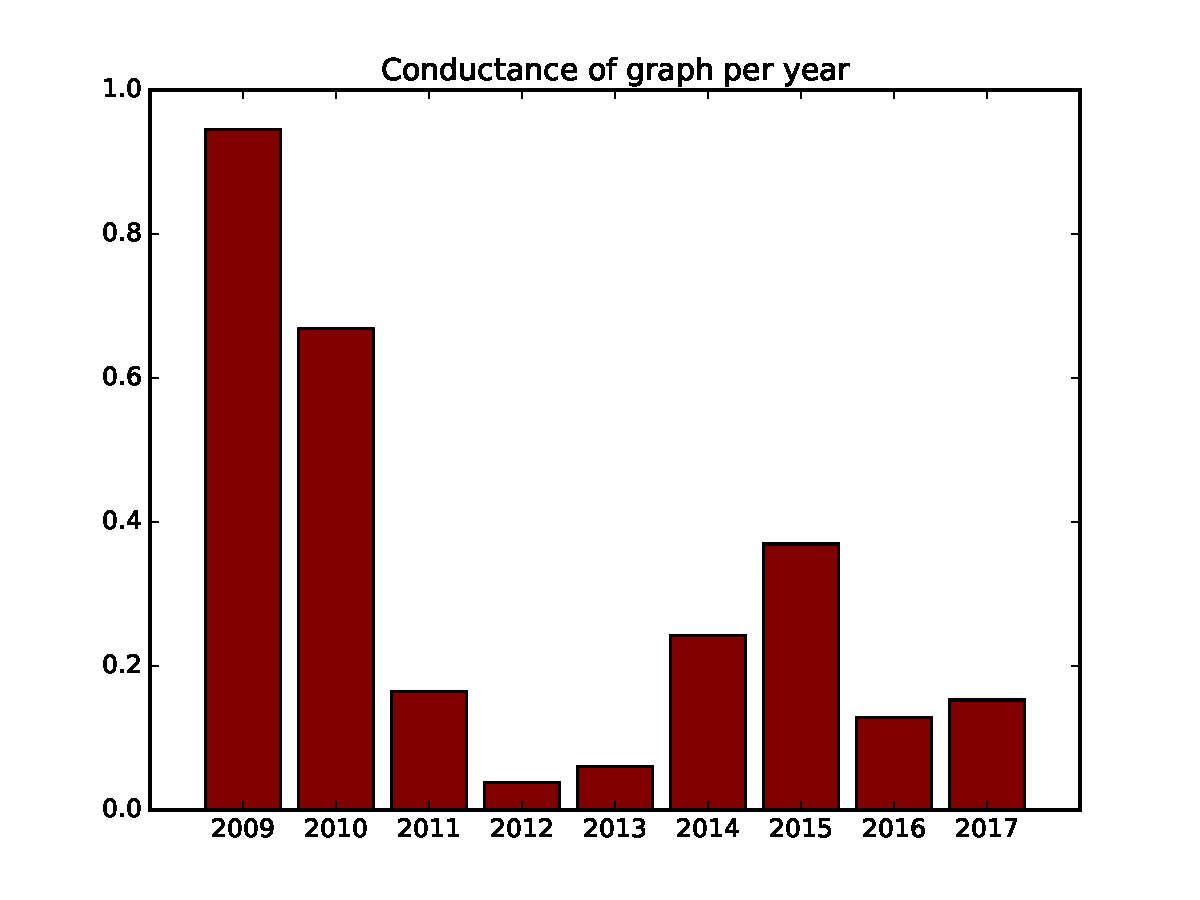
\includegraphics[width=1\linewidth]{./images/conductance}
	\centering
	\caption{The Conductance of 10 communities of the graph for each year from 2009 until March of 2017. The years 2009 and 2010 have the highest ratio thus in those two years the graph was not well isolated and had some bottleneck. The years 2012 and 2013 show that the graph was diverse. In general for most of the years the conductance is far below the half which is a sign of good clustering.}
	\label{fig:fig6}
\end{figure}

\begin{figure}[h!]
    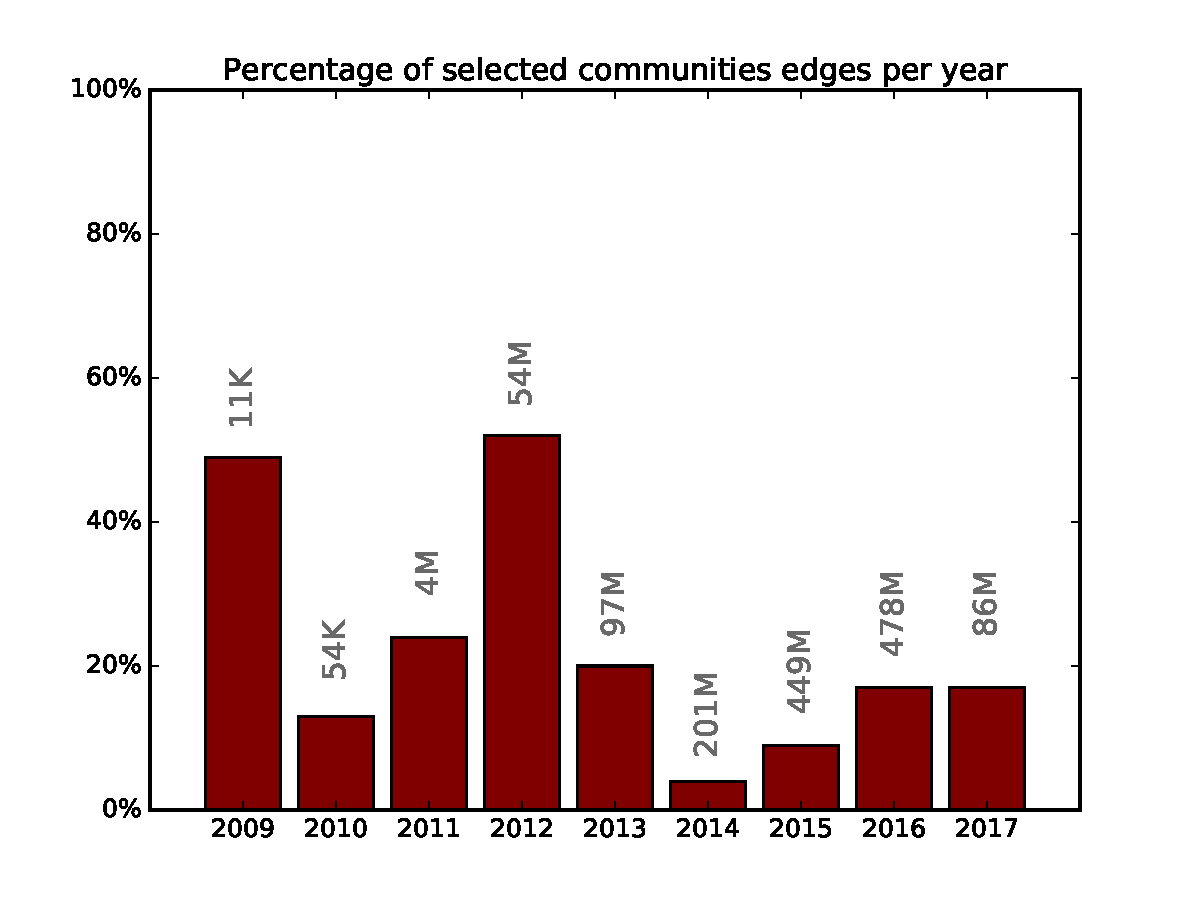
\includegraphics[width=1\linewidth]{./images/edgePercentage}
	\centering
	\caption{To compute conductance we select the top 10 communities with the highest number of edges. The chart shows the percentage and the number of the selected edges of the communities proportional to the total edges of the graph for each year from 2009 to March 2017.}
	\label{fig:fig7}
\end{figure}





\subsection{Bridge Ratio and Diameter}
As we further discuss later in~\secref{sec:discussion}, our computations are
heavy and as the size of the graph increases the more trivial it becomes to
obtain a result, especially for the Bridge Ratio and the Diameter. Hence, we
are not able to have a complete image as those metrics are concerned. 

For the Bridge Ratio we are able to obtain a result only for 2009 as an annual image and for 2009-2010 for the months. The reported result for 2009 is that 24\% of the edges are bridges, however we cannot reach to any conclusion. As the Diameter is concerned, the result that we obtain for both years and months is for 2009, which is \textit{Infinity} in both cases and the meaning is that the graph has disconnected components.



\section{Discussion}
\label{sec:discussion} 
Our approach to analyze structure evolution of the Bitcoin Blockchain 
focuses on comparison between each year treating it as an individual transactions
graph. That kind of approach does not provide a clean image though for the evolution over the years,
however computing the metrics by taking into account also each
previous year, is not feasible as the size of the graph increases dramatically. The computations are very heavy and 
we lack of computational power. We faced many difficulties to compute most of the metrics even
with our approach. Although we could not manage to master all the technical
difficulties, we tried to approach them by making optimizations, using more of the available
resources, trying different implementations and configuring Spark. We struggled
a lot with Diameter, Bridge Ratio, Average Clustering Coefficient and
Conductance. Our jobs never produced any results after more than 8 hours of
running or failed due to memory exceptions. For each individual computation we
used 100 executors with 1 core and 10GBs of memory per each. We even tried to
increase the amount of given resources in late hours where the cluster was not
used by other teams, however 8 hours in most cases were not enough to
compute not even the results for 2009 which is the smallest graph. Generally,
the graphs have a size class of some MBs except from 2014
till 2016 that are some GBs. 

From the Spark logs we observed that in some cases the Average Clustering Coefficient failed due to memory and the issue was data locality. It appeared that in certain stages when an executor was assigned a task whose input was not stored locally, the executor would fetch the block from a remote executor where the block was present. This block was then materialized in memory heap until the task was completed. Hence, to avoid the out of memory errors we should just increase the heap size so that remote blocks can fit. That kind of memory increment is huge enough and practically impossible with our available resources. Thus, we tried to use some partition strategies that GraphX provides but the result at the end was the same. Since we could not obtain the results, we asked the help of our colleague at the Institute of Computer Science of Foundation for Research and Technology Hellas (ICS-FORTH), who was able to compute it for the years 2014-2016 in a cluster of 7 machines with 32 cores and 256GBs of memory each.

Computing the Diameter for 2009 and for each month of 2009 took 12 hours for a graph that does not exceed 5 MBs as a parquet file with a total size of 22.000 edges. Instead of using the open-source algorithm we also tried to create our own by using GraphFrames that are much faster than the traditional RDDs. Even though we had some kind of improvement, the job for 2010 was running about 5 hours and still no results were produced. 

To compute Bridge Ratio we followed two approaches. The first one was of a high complexity as we tried to find the bridges by removing one edge at a time while checking if the number of connected components was inscreasing. If it did, that edge was a bridge. Our second approach is an algorithm derived from a C++ implementation~\cite{geeksForGeeks} that uses DFS in order to find the bridges on the graph. Like Diameter, finding bridges took also more than 8 hours for 2009. For 2010 after a certain point we got a stack-overflow exception due to the recursion that we use in our implementation. We then increased the stack to 1GB by using the -Xss on runtime. Even though the problem seemed to be solved, after 11 hours we did not have any result for 2010.


For both Bridge Ratio and Diameter we tried to eliminate as much as possible the computations needed by removing the duplicate edges. Those edges as we refer in~\secref{sec:implementation}, are coming from the join between the input and the output transactions. Since the Bride Ratio and Diameter are based on finding shortest paths, duplicate edges increase the complexity of the computation, while removing them does not change the final results at all. However neither this elimination helped the situation as the algorithms were still running for many hours without results, and since we had other concerns we did not spend more time on that.

In order to compute Conductance we transform the graph into communities by using the \textit{Label Propagation} algorithm that is already implemented in GraphX. We performed some experiments on the graph of 2016, since it is the largest, and for 25 iterrations the process took 8 and a half hours while for 10 iterations, took almost 4, so this is another bottleneck. In addition, the computation of Conductance after forming the communities was also very time consuming and hence, we followed the process described in \secref{sec:implementation}. Choosing only 10 communities to perform the computations for conductance was not our intention. With our setup and the constraints in the number of iterations for the \textit{Label Propagation}, computing Conductance took 35 hours and 30 minutes for years and the same for months. Finally, in our website~\cite{website}, we have created graph visualizations for the community that had the minimum Conductance, hence the Conductance of the graph. However, those visualizations are until 2011. The reason behind is the file size of the edges. For 2012 the size of the file is 800MBs while for 2013 it is more than 1GB. We measured the memory needed by Gephi on our local machines in order to load the file for 2013. Unfortunately, 10GBs of RAM were not enough and we were not able to load the graph and export the .gexf files for preview at our website.
\section{Related Work}
\label{sec:related}
During the past 9 years, from the creation of the Bitcoin Blockchain, there is a variety of analysis from many different aspects. Ron et al.~\cite{Ron}, have made a Quantitative Analysis of the full Bitcoin Blockchain transactions graph. However, their work differentiates from ours in terms of analysis. They are mainly focusing on exchange issues among users and they also deepen in the relation between transactions. On the other hand, McGinn et al.~\cite{McGinn} focus on activity of the transactions between users by providing a variety of interesting visualizations. They observe high frequency transaction patterns but also an uptrend of the Denial-of-Service-Attacks on the Bitcoin network. Even though their work is not relevant with ours in terms of graph-computations, they provide us very useful information about the transactions of Bitcoin.

The work from Bakayov and Custura~\cite{Bakayof} is in the same vein with ours but we approach the problem differently and compute different metrics. Moreover, they take into account the graph as a whole and they do not compute each year individually, which is a common-sense approach. However, most of their computations are not so heavy and except from Harmonic Centrality, they work with officialy optimized implementations maintained by the contributors of GraphX. 

Despite the fact that many researches are not about the Bitcoin Blockchain graph, they are also focusing on graph analysis and statistics. Quick et al.~\cite{Quick} compute also the Diameter and the Clustering Coefficient among other metrics. However, their work focuses on Social Network Analysis using Pregel-like large scale graph processing frameworks. They present several undirected graph algorithms for Social Network analysis and furthermore discuss various graph componentisation methods.

Finally, another approach is the one by Prat-Perez et al.~\cite{PratPerez} who compute metrics similar to ours but they are based on community-like analysis. Following their way we could split the graph of each year into communities by using the \textit{Label Propagation}, divide the communities in categories by size, discard communities with real small size and take a weighted sample from each size category. Such an approach would lead to a distribution of each metric very similar to the results if we have made the computation for the whole graph.

\section{Conclusions and Future Work}
\label{sec:conclusions}

The purpose of our work is to provide an insight of the evolution of the
Bitcoin Blockchain transactions graph. To achieve this, we analyze 98GBs of
data from which we keep only the necessary for the creation of the edges for each graph, managing 
to reduce them to 14GBs of parquet files. We split the whole graph
into subgraphs for each year and then for each month, so we can compute several
indicative for-the-graph metrics on certain time snapshots. Then, we create the
analogous visualizations which we upload at our website~\cite{website}. Our
results show that the graph tends to increase progressively each year, reaching
a peak in 2015. From the results it is obvious that since 2011 the activity of
the network was intense. However, we do not have a compelete image for 2017,
since our data are until March. 

Engaging with such a large graph-dataset makes the usage of Spark in
combination with GraphX decisive as they allow us to compute several metrics,
providing the necessary tools for graph processing. However, Bridge Ratio and
Diameter are too heavy computations and expensive algorithms. As the size of
the graph per year increases to billion edges, those tools we had in our
pleasure did not manage to provide any results, probably due to the lack of computation
power. 

As a future work we would like to approach the Bitcoin Blockchain graph in community analysis as described in the last paragraph of~\secref{sec:related}. This approach seems to apply better on large graphs and probably it would be faster to obtain the desired results. 
\section{Acknowledgments}
First of all, we would like to express our gratitude to Professor Peter Boncz not only for his help and advices during our work,
but also for the chance to obtain hands on experience dealing with real-world big data problems.

We would also like to thank Iakovos Kolokasis from the Institute of Computer Science of Foundation for Research and Technology Hellas (ICS-FORTH),
for helping us understand some complex parts of the graph theory and also for computing the results of the Local Clustering Coefficient from 2014 until 2016.

This work was carried out on a small part of the Dutch national e-infrastructure with the support of SURF Cooperative.


\section{Work Distribution}
\textit{Metrics implementation:}
\begin{itemize}[noitemsep,topsep=0pt]
\item \textbf{Maria:} Size, TPR, Bridge Ratio, Diameter (open-source)
\vspace{1mm}
\item \textbf{Thodoris:} Conductance (half), Global Clustering Coefficient, Local Clustering Coefficient (open-source)
\vspace{1mm}
\item \textbf{Manuel:} Bridge Ratio (try), Conductance (half)
\end{itemize}
\vspace{2.5mm}
\textit{Visualization:}
\begin{itemize}[noitemsep,topsep=0pt]
\item \textbf{Maria:} Report visualizations
\item \textbf{Thodoris:} Website visualizations
\end{itemize}
\vspace{2.5mm}
\textit{Report:}
\begin{itemize}[noitemsep,topsep=0pt]
  \item \textbf{Maria}
  \item \textbf{Thodoris}
\end{itemize}


{\footnotesize 
	\bibliographystyle{acm}
	\bibliography{paper}
}

%\theendnotes

\end{document}
